\section{Evaluation} \label{section:evaluation}

\subsection{Single Hop}

\begin{figure}[t]
\centering
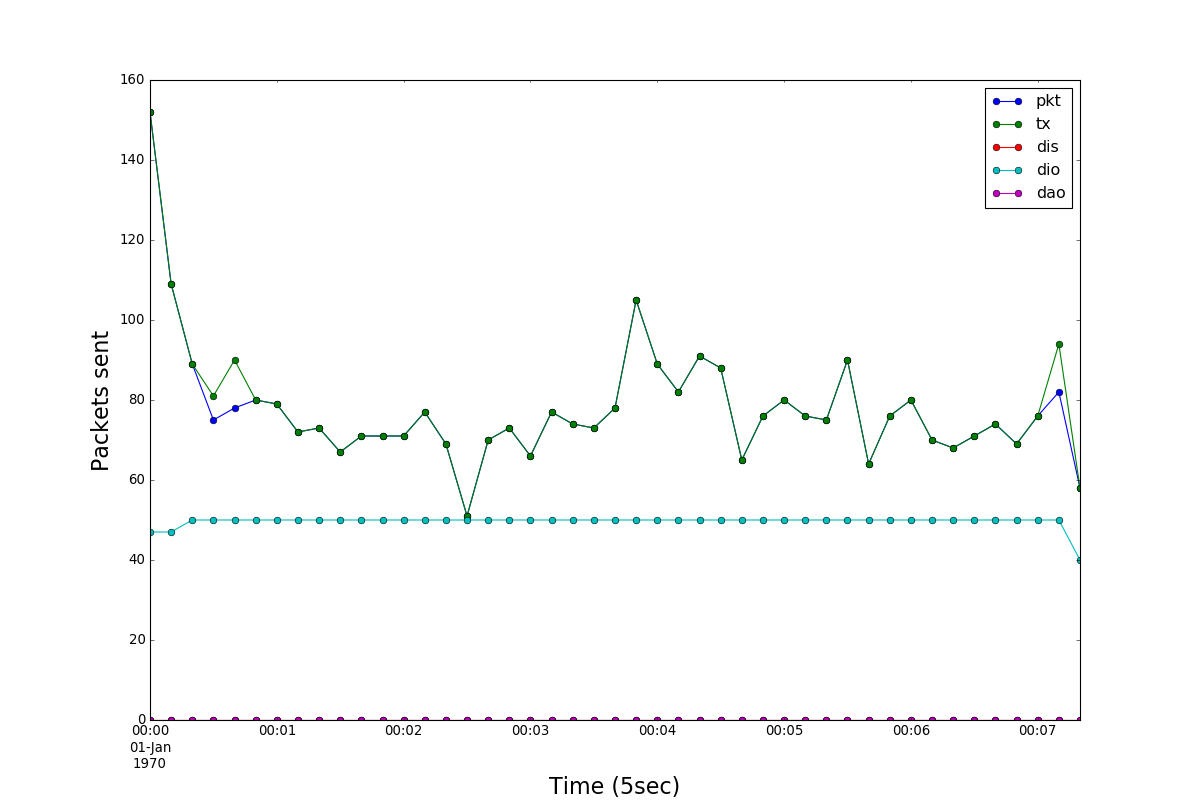
\includegraphics[width=\linewidth]{figs/rpl_single_hop.png}
\caption{Packet types sent over time in a RPL topology of a single broadcast domain.}
\label{fig:rpl_single_hop}
\end{figure}

\begin{figure}[t]
\centering
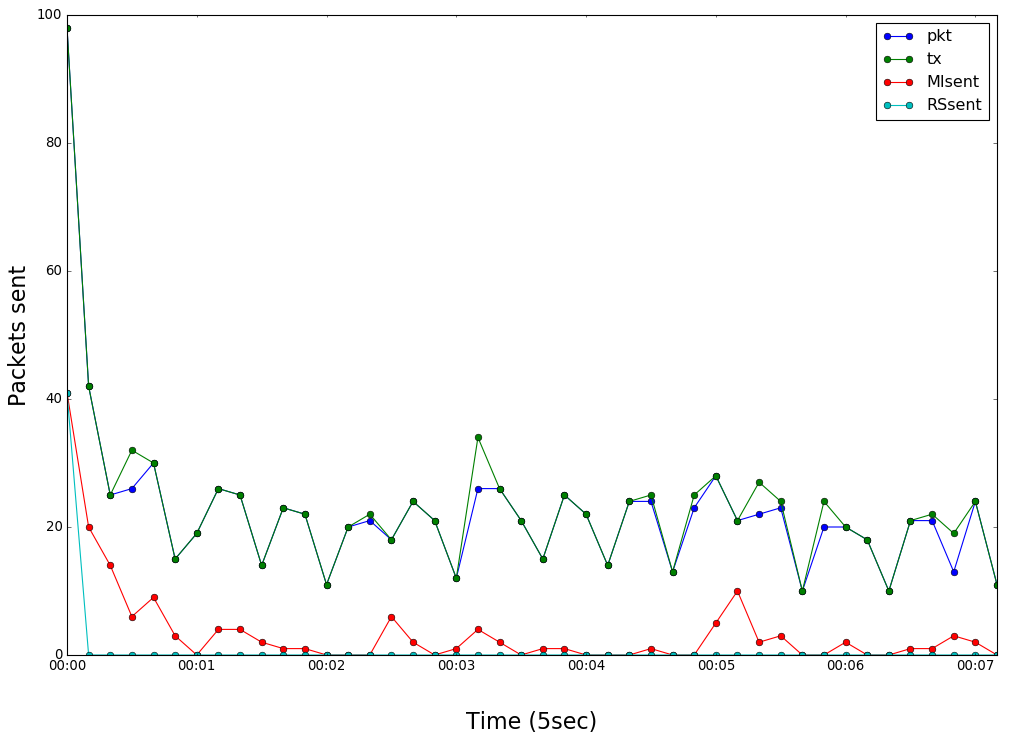
\includegraphics[width=\linewidth]{figs/3hop_single_hop.png}
\caption{Packet types sent over time in a 3hop topology of a single broadcast domain.}
\label{fig:3hop_single_hop}
\end{figure}

\begin{table}
\centering
\caption{Summary of the results from the four network scenarios using both RPL and 3hop in a single broadcast domain deployment and a multihop deployment}
\label{table:results}
\begin{tabular}{|l|l|l|l|}
\hline
\textbf{Experiment} & \textbf{Reported/Total} & \textbf{PRR min/max} & \textbf{PRR mean/std} \\
\hline
\hline
RPL Single Hop & 10 / 10 & 36\% / 100\% & 82\% / 21\% \\
3hop Single Hop & 10 / 10 & 97\% / 100\% & 98\% / 1\% \\
RPL Multi Hop & 8 / 10 & 48\% / 51\% & 50\% / 1\% \\
3hop Multi Hop & 10 / 10 & 86\% / 100\% & 95\% / 4\% \\
\hline
\end{tabular}
\end{table}

\if 0
Want to evaluate the code dissemination part

Describe the methodology:
- what are the aspects of routing protocol we find important, i.e. what are our goals
- given these goals, what do we need to evaluate to demonstrate whether or not we achieved them
- probably want to write the RPL/ipv6 nd discussion first
\fi
